\section{Ransac mit Maskierung}

% Textumflossenes Bild des ''Ringfilter''-Kerns
\begin{wrapfigure}{r}{0.5\textwidth}
 \centering
  
\includegraphics[width=0.3\textwidth]{fahrspurerkennung_ransac_midfilter.png}
  \caption{Der Kern des ''Ringfilters''}
\label{fig:fahrspurerkennung_ransac_midfilter}
\end{wrapfigure} 

Der nun folgend beschriebene Ansatz zur Detektion der Fahrbahnlinien ist in der endgültigen Implementierung nicht zum Einsatz gekommen. Da wir uns jedoch lange Zeit damit beschäftigt und viele später weiter verwendete Grundfunktionen aufgebaut haben, wird die Vorgehensweise nun näher erläutert.
Die Implementierung begann bereits vor Fertigstellung der Hardware. Zu jenem Zeitpunkt ist deshalb der Bildausschnitt noch nicht so, wie in~\ref{fig:bildvorverarbeitung_entzerren} zu sehen, gewählt worden, weshalb die Abbildungen~\ref{fig:fahrspurerkennung_ransac_binarisieren}, ~\ref{fig:fahrspurerkennung_ransac_masken} und~\ref{fig:fahrspurerkennung_ransac_ransac} einen anderen Teilbereich darstellen. Das ändert indes nichts an dem Algorithmus selbst, sondern ist nur eine Sache der Parametereinstellungen. 


% entzerrtes und binarisiertes Beispielbild und Filterergebnisse für Mittellinie nebeneinander
\begin{figure}[H] % [htb]
  \centering
  \subfloat[][]{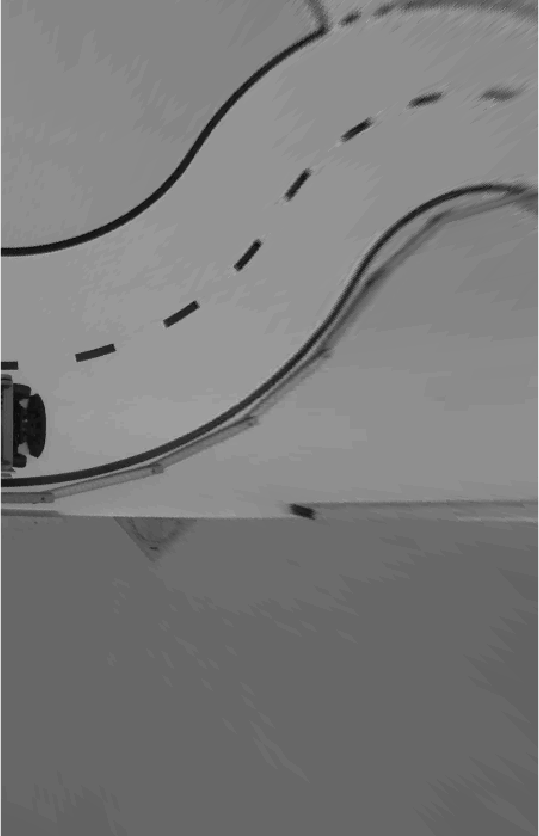
\includegraphics[width=0.35\textwidth]{fahrspurerkennung_ransac_imgUndist.png}}
  \qquad \quad
  \subfloat[][]{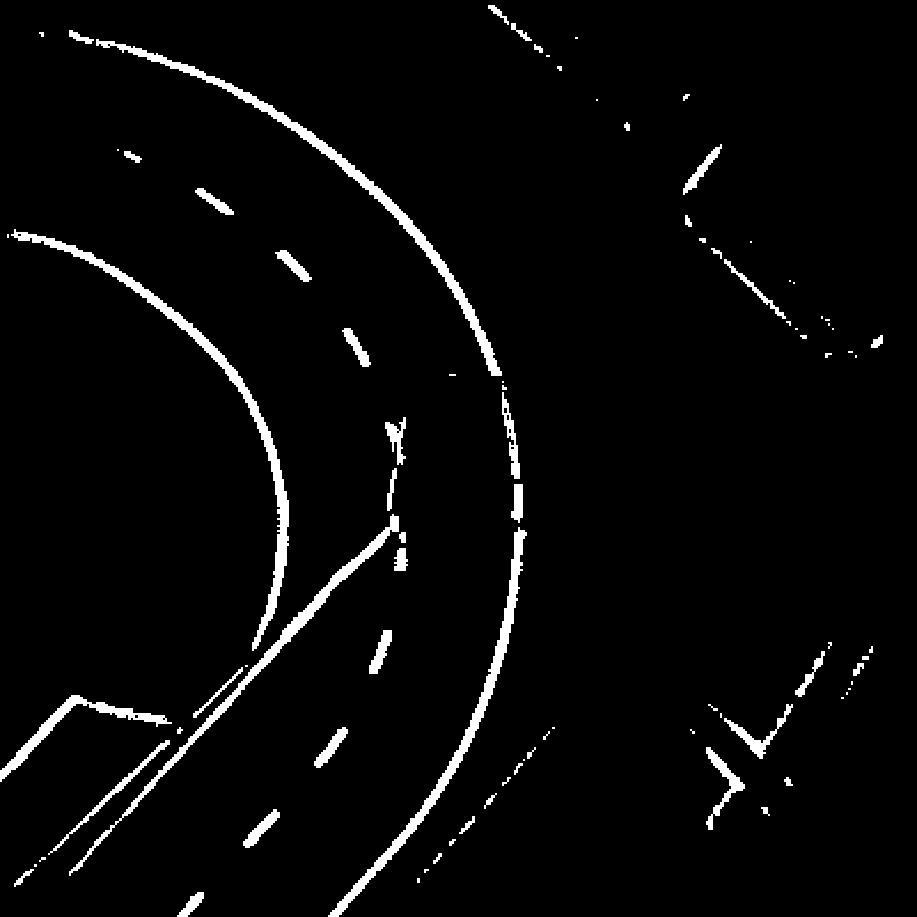
\includegraphics[width=0.35\textwidth]{fahrspurerkennung_ransac_imgBinarized.png}}
  \qquad \quad
  \subfloat[][]{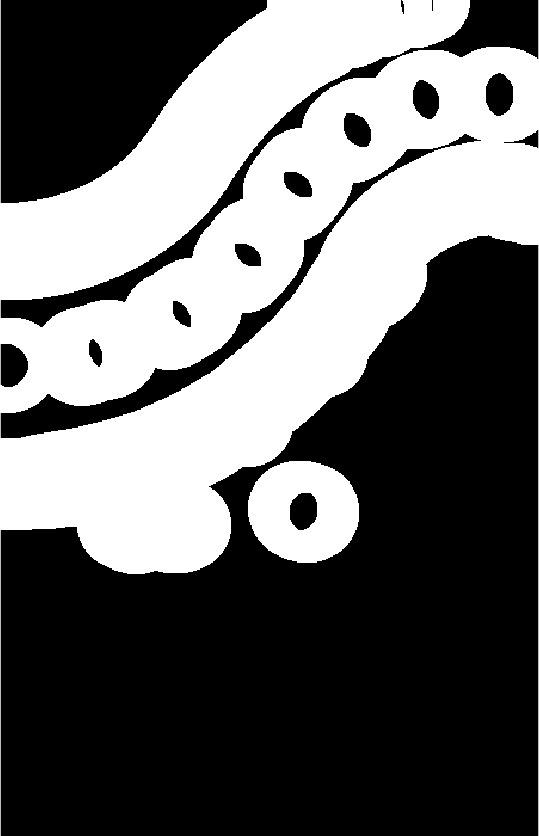
\includegraphics[width=0.35\textwidth]{fahrspurerkennung_ransac_imgMidFiltered.png}}
  \qquad \quad
  \subfloat[][]{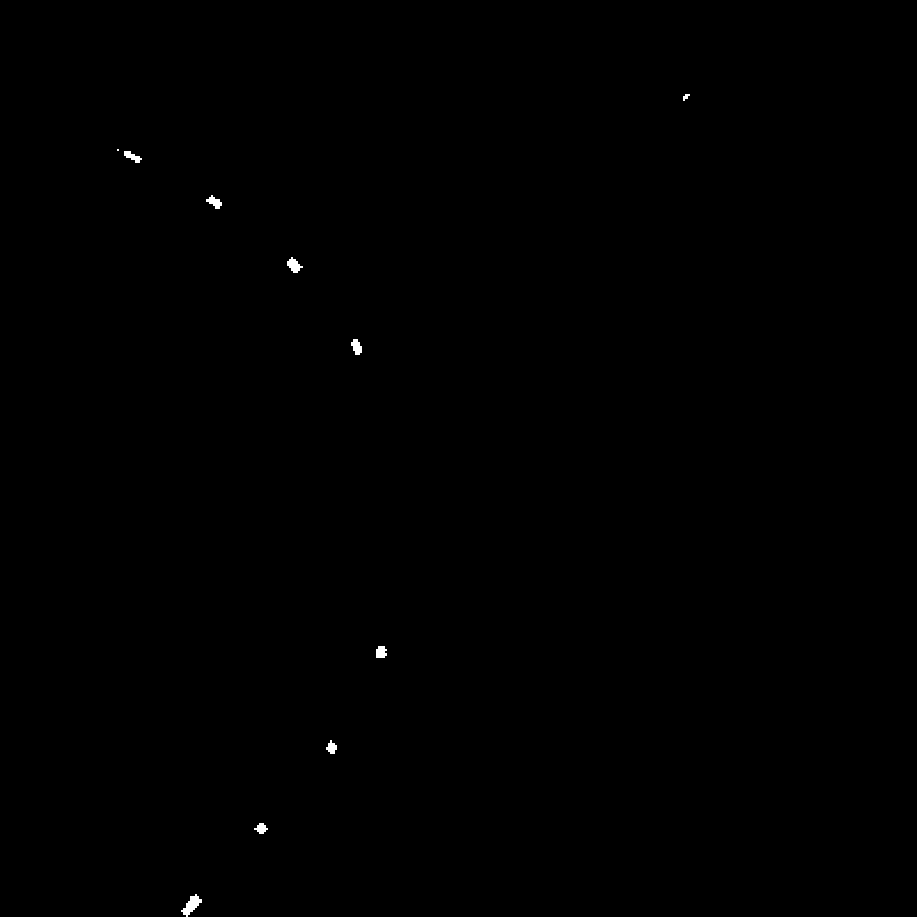
\includegraphics[width=0.35\textwidth]{fahrspurerkennung_ransac_imgBinarizedAndNotImgMidFiltered.png}}
  \caption{entzerrtes (a) und binarisiertes Bild (b) einer Testaufnahme auf der Strecke in alten Einstellungen; Filterergebnis des ''Ringfilters'' (c) und Duchschnitt dessen Negation mit dem binarisierten Bild (d)}
\label{fig:fahrspurerkennung_ransac_binarisieren}
\end{figure} 



% Bilder der drei Masken für linke, mittlere und rechte Linie
\begin{figure}[H] % [htb]
  \centering
  \subfloat[][]{
\includegraphics[width=0.3\textwidth]{fahrspurerkennung_ransac_imgMaskLeft.png}}
  \quad
  \subfloat[][]{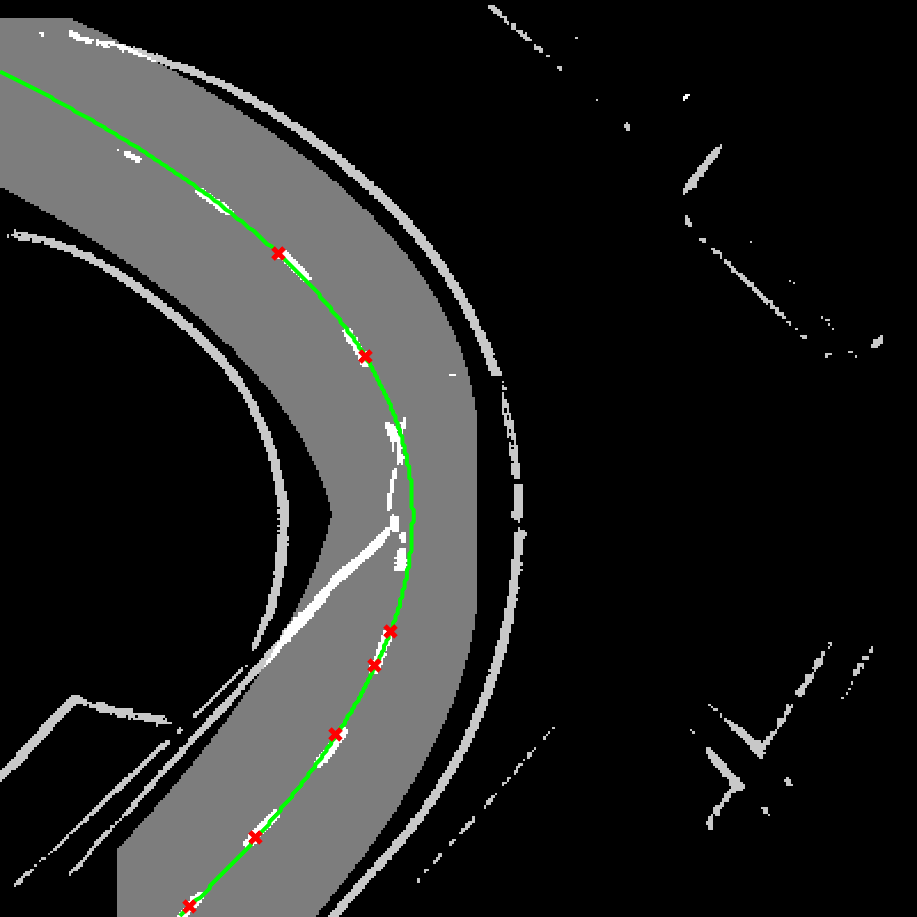
\includegraphics[width=0.3\textwidth]{fahrspurerkennung_ransac_imgMaskMiddle.png}}
  \quad
  \subfloat[][]{
\includegraphics[width=0.3\textwidth]{fahrspurerkennung_ransac_imgMaskRight.png}}
  \caption{Masken zum Herausschneiden der linken (a), mittleren (b) und rechten Fahrbahnmarkierung für die Anwendung des \gls{acr:ransac}-Algorithmusses}
\label{fig:fahrspurerkennung_ransac_masken}
\end{figure} 

% Bilder der drei Ausführungen des RANSAC für linke, mittlere und rechte Linie
\begin{figure}[H] % [htb]
  \centering
  \subfloat[][]{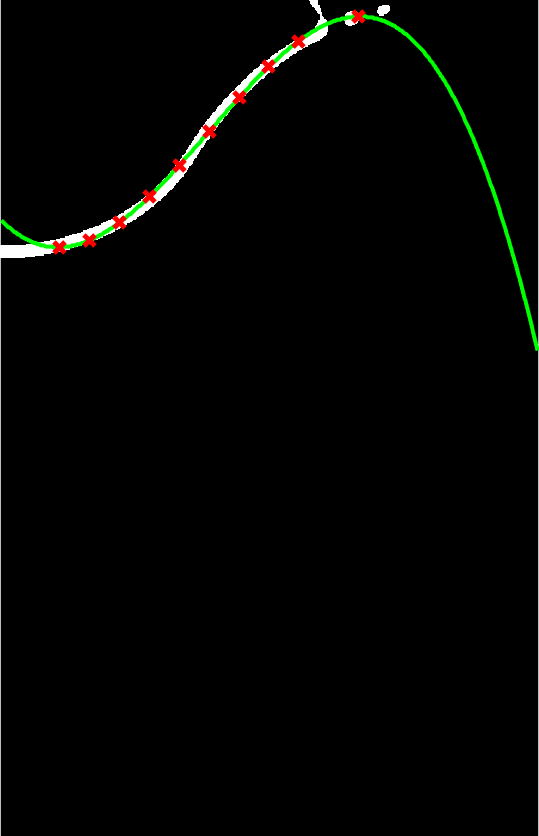
\includegraphics[width=0.3\textwidth]{fahrspurerkennung_ransac_imgRansacLeft.png}}
  \quad
  \subfloat[][]{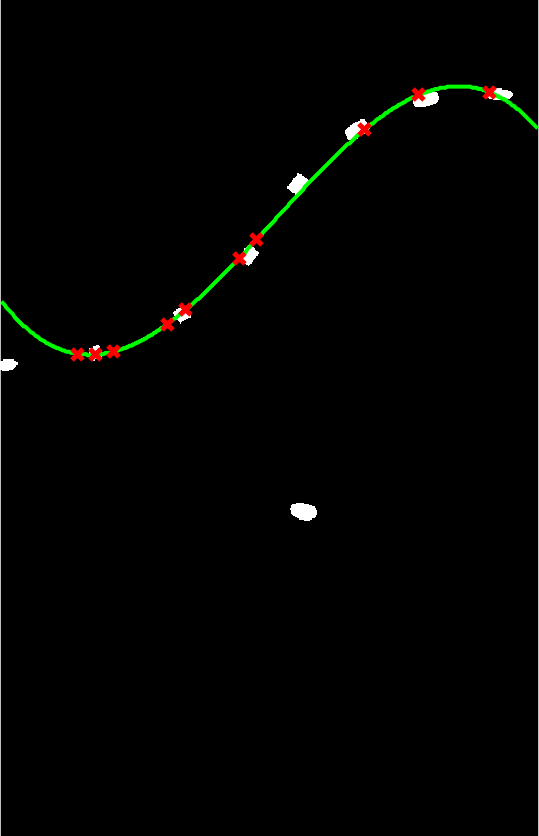
\includegraphics[width=0.3\textwidth]{fahrspurerkennung_ransac_imgRansacMiddle.png}}
  \quad
  \subfloat[][]{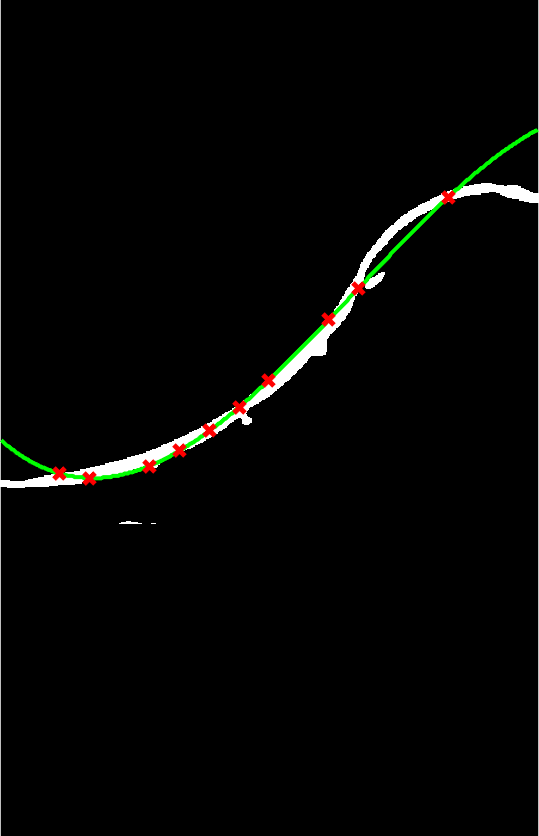
\includegraphics[width=0.3\textwidth]{fahrspurerkennung_ransac_imgRansacRight.png}}
  \caption{Approximation der linken (a), mittleren (b) und rechten Fahrbahnmarkierungen durch eine Funktion dritten Grades mittels \gls{acr:ransac}}
\label{fig:fahrspurerkennung_ransac_ransac}
\end{figure} 

% Bild/Plot der eingetragenen Punkte in der Weltkarte
\begin{figure}[H] % [htb]
  \centering
  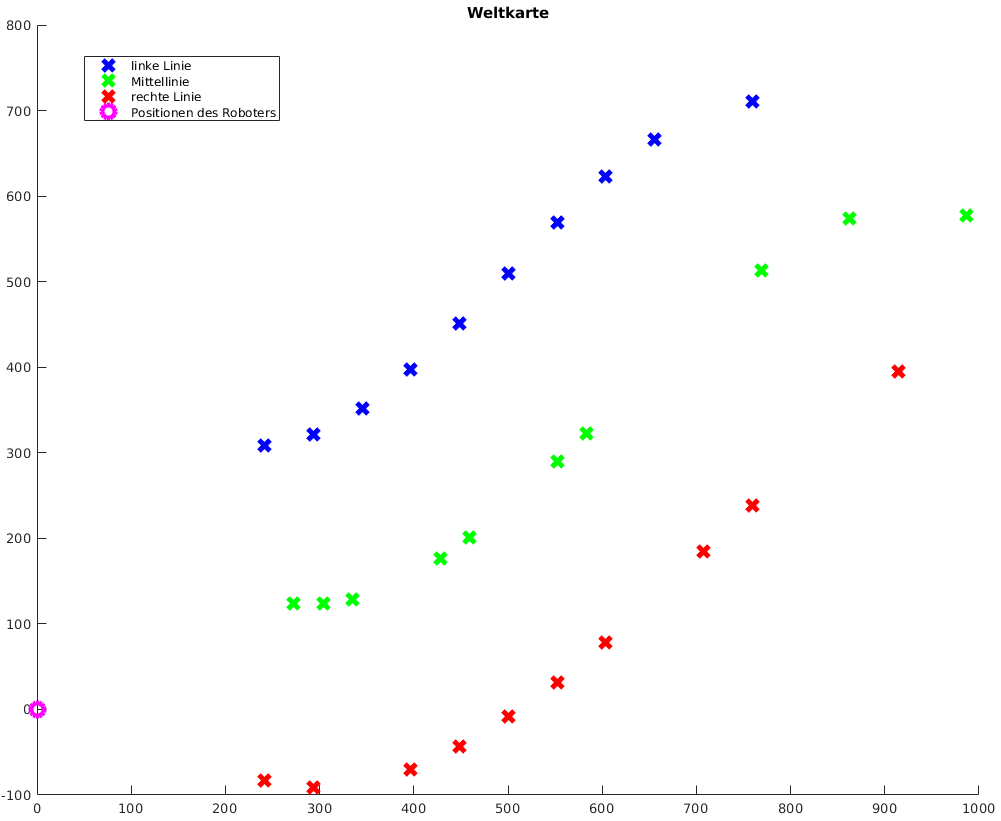
\includegraphics[width=0.9\textwidth]{fahrspurerkennung_ransac_plotWorldMap.png}
  \caption{Plot der eingetragenen Punkte in die Weltkarte}
\label{fig:fahrspurerkennung_ransac_karte}
\end{figure} 

